\documentclass{article}

\usepackage[letterpaper,top=2cm,bottom=2cm,left=3cm,right=3cm,marginparwidth=1.75cm]{geometry}
\usepackage[T1]{fontenc}
\usepackage{appendix}
\usepackage{authblk}
\usepackage{authblk}
\usepackage{amsmath, amsfonts, amssymb}
\usepackage{graphicx}
\usepackage{algorithm}
\usepackage{amsthm}
\usepackage{bm}
\usepackage{cases}
\usepackage{caption}
\usepackage{xr-hyper}
\usepackage{hyperref}
\usepackage{xurl}

\DeclareMathOperator*{\argmin}{argmin}
\DeclareMathOperator{\short}{sh}
\DeclareMathOperator{\Ex}{\mathbb{E}}


\usepackage{setspace}
\singlespacing

\usepackage{parskip}

\usepackage{soul}
\usepackage{xcolor}
\def\elr#1{{\color{cyan}\textbf{ELR:[#1]}}}
\def\apg#1{{\color{red}\textbf{APG:[#1]}}}
\def\bwr#1{{\color{violet}\textbf{BWR:[#1]}}}
\def\ngr#1{{\color{blue}\textbf{NGR:[#1]}}}

\usepackage{natbib}
\bibliographystyle{rss-abbr}


\author{Aaron Gerding\thanks{Corresponding Author: \texttt{agerding@umass.edu}}}
\author{Nicholas G. Reich}
\author{Benjamin Rogers}
\author{Evan L. Ray}
\affil{Department of Biostatistics and Epidemiology, School of Public Health and Health
Sciences, University of Massachusetts at Amherst}

\title{Evaluating infectious disease forecasts \\ with allocation scoring rules}

\usepackage{Sweave}
\begin{document}
\input{manuscript-concordance}

\newcommand{\del}[2]{\frac{\partial {#1} }{\partial {#2}} }
\newcommand{\dby}[2]{\frac{d {#1} }{d {#2}} }
\newcommand{\sbar}{\overline{s}}
\newtheorem{proposition}{Proposition}

\theoremstyle{remark}
\newtheorem*{remark}{Remark}

\maketitle




\begin{Schunk}
\begin{Sinput}
> library(targets)
> library(tidyverse)
> library(ggbump)
> theme_set(theme_bw())
> ## necessary to have project root as wd, to override document directory
> knitr::opts_knit$set(root.dir = '../')
\end{Sinput}
\end{Schunk}

\begin{abstract}
Recent years have seen increasing efforts to forecast infectious disease burdens, with a primary goal being to help
public health workers make informed policy decisions. However, there has only been limited discussion of how
predominant forecast evaluation metrics might indicate the success of policies based in part on those forecasts. We
explore one possible tether between forecasts and policy: the allocation of limited medical resources so as to minimize
unmet need. We use probabilistic forecasts of disease burden in each of several regions to determine optimal resource
allocations, and then we score forecasts according to how much unmet need their associated allocations would have
allowed. We illustrate with forecasts of COVID-19 hospitalizations in the US, and we find that the forecast skill
ranking given by this allocation scoring rule can vary substantially from the ranking given by the weighted interval
score. We see this as evidence that the allocation scoring rule detects forecast value that is missed by traditional
accuracy measures and that the general strategy of designing scoring rules that are directly linked to policy
performance is a promising direction for epidemic forecast evaluation.
\end{abstract}

\noindent \textbf{Keywords:} public health, forecast evaluation, proper scoring rules, resource allocation, epidemiology

\section{Introduction}

Infectious disease forecasting models have emerged as important tools in public health outbreak response. The
predictions they provide increasingly inform decisions regarding a wide variety of countermeasures intended to reduce
transmission and mitigate the severity of disease outcomes. For example, estimates of the onset time of the flu season
have been used in developing national vaccination strategies \citep{igboh2023timing}, and forecasts of Ebola and
diptheria dynamics have been made with the clearly stated goal of helping local public health workers choose the timing
and location of interventions in settings where resources are severely constrained 
\citep{meltzer2014estimating, rainisch2015regional, camacho2015-ebola-bed,finger_real-time_2019}. More recently, in the
context of the outbreak of COVID-19 across the US, \cite{bertsimas2021predictionsCOVID} used forecasts as inputs to
decision tools for the interstate reallocation of ventilators and ICU capacity, and to recommend vaccine trial sites to
a major trial sponsor. \cite{fox_real-time_2022} similarly used predictive models to inform intrastate resource and
care site planning, as well as local community guidelines for masking, traveling, dining and shopping (University of
Texas, 2022)\nocite{utnews2022}.

In the wake of the COVID-19 pandemic, this trend has been followed by calls for infectious disease forecasts to be not
only designed, but also evaluated in ways that align specifically with how forecasts can be used to inform such outbreak
control decisions \citep{marshall2023predictions, bilinski_adaptive_2023}. This contrasts, however, with the
historically standard practice of measuring the quality of disease forecasts using general purpose accuracy and skill
scores, especially those that have implementations available in existing software when the relevant outbreak occurs. For
point forecasts, the root mean square error (RMSE) (e.g., \cite{papastefanopoulos2020covid}) and the mean absolute error
(MAE) (e.g., \cite{johansson2016evaluating}) are common choices. For probabilistic forecasts, which are the focus of
this paper, researchers have often relied on the logarithmic score (LS). For example, the LS has been used to evaluate
the skill of US seasonal influenza forecasts \citep{mcgowan_collaborative_2019,reich_collaborative_2019} as well as
forecasts targeting surveillance measures of dengue incidence in Peru and Puerto Rico \citep{johansson_open_2019}. More
recently, the continuous ranked probability score (CRPS) and a discretized version adapted to multi-quantile forecasts,
the weighted interval score (WIS) \citep{bracher2021evaluating}, have gained prominence. For example, the CRPS was used
to assess probabilistic forecasts (based on random effect models) of dengue incidence at the district level in Vietnam
\citep{colon-gonzalez_probabilistic_2021}. Likewise, the WIS has been used during the COVID-19 pandemic to evaluate forecasts
of observed cases, hospitalizations and deaths in the US and Europe, as reported by municipal, state, and federal
surveillance systems \citep{cramer_evaluation_2022,fox_real-time_2022,sherratt2023predictive}.

While any of these scores can be interpreted through the lens of decision theory, they lack explicit connections between how a forecast is evaluated and how that forecast was used in practice. A key impetus for the present work was to develop a score that is interpretable to decision makers by measuring the extent to which forecasts lead to improved decisions. In addition, the allocation score we propose is expressed in units that are intelligible to decision makers.

A general phenomenon at play here --- one that has been observed repeatedly over the past few decades in other fields
such as finance, supply chain management, and meteorology --- is that while scores such as RMSE, MAE, LS, CRPS, and WIS
can describe the \emph{quality} of a forecast in terms of how well it corresponds to the observed disease outcome, they
will often fail to register the \emph{value} of a forecast in the context of a specific decision. We refer the reader to
\cite{yardley2021utility_cost_forecasts} and the references collected therein (especially the foundational
\cite{murphy1993whatisagoodforecast}) for a general overview touching on a wide range of forecasting contexts and  also
to \cite{pesaran2002decision_based_eval} for a clear discussion from an econometric perspective.

Despite this now well-developed discussion of the quality-value distinction in the larger forecasting community, we are
aware of only a limited literature attempting to connect the value of \emph{infectious disease} forecasts to their
impact on and through policy.  Even within this body of work we have found the discussion of such a connection to
be at a formally and quantitatively imprecise stage. In \cite{ioannidis2022forecastingCOVIDfailed}, the possible negative
consequences of inaccurate forecasts of infectious disease are discussed, but there is no attempt to quantify the
utility or loss incurred as a result of those forecasts. \cite{bilinski_adaptive_2023} explore ways in which predictive
classifiers of local COVID-19 risk levels in the US could be tuned to policymaker preferences for different costs
associated with over- and under-reaction to disease dynamics, but they do not clearly identify the source of these
costs or how they depend on quantifiable policy choices. A similar discussion related to dengue countermeasures in
Vietnam appears in \cite{colon-gonzalez_probabilistic_2021}.  A novel version of the WIS informally motivated by
utility considerations is developed in \cite{marshall2023predictions}, but the score is not derived in a
decision-theoretic manner.  There is also a thread of literature that frames infectious disease modeling as a component
of a larger system for understanding how policy goals, means, and choices interact and constrain one another. As an
example, \cite{Probert2016decisionMakingFootMouth} explore how policy recommendations ought to flow from a possibly 
incongruous set of simulation-based projection models of a hypothetical foot-and-mouth disease outbreak when there are 
ranges of plausible responses and stakeholder interests. Decision theory plays a prominent role here, but not explicitly
as a way to evaluate the choices made in developing the models.

In this work, we begin to fill this gap between the ways that infectious disease forecasts have traditionally been
evaluated and the ways that they have been used to support public health policy. To do so, we consider a setting in
which forecasts are used to help determine the allocation of a limited quantity of medical supplies across multiple
regions. In section~\ref{sec:methods} of the paper, we define a new forecast scoring rule --- the {\em allocation score}
--- that evaluates forecasts based on how beneficial resource allocations derived from them would turn out to be. In
section \ref{sec:application}, we present an illustrative analysis using the allocation score to evaluate forecasts of
hospital admissions in the US that were made leading up to and during the Omicron wave that peaked in January of 2022.
This analysis is ``synthetic'' insofar as it is not intended to correspond to any specific historical record of
allocation decisions that could have been supported by hospitalization forecasts during this period. However, we view
the general allocation problem on which our framework is based as a versatile template for formalizing real-world
decisions that must constantly be made in real-time by public health administrators around the globe, especially those
related to hospital capacity, ventilator usage, doses needed for specific medications and other situations where an
outbreak creates sudden and highly variable demand for potentially scarce resources.  

\section{The Allocation Score}
\label{sec:methods}

We begin with an informal description of the allocation score and some examples illustrating its key characteristics in
section \ref{sec:methods.overview}. In section \ref{sec:methods.detailed} we develop the allocation score more
carefully, using a decision theoretic procedure for deriving proper scoring rules. (See appendix \ref{sec:a:proper}
for a definition of a proper scoring rule and a more technical discussion of the procedure). In section
\ref{sec:methods.related}, we note that another group of common scores including the quantile score, WIS, and CRPS, can
also be derived from decision theoretic foundations \textemdash starting from a different decision making context.

\subsection{Overview of Allocation Scoring}
\label{sec:methods.overview}

Suppose that a decision maker is tasked with determining how to allocate $K$ available units of a resource across $N$
locations. If the decision maker is provided with a multivariate forecast $F$ where each marginal forecast distribution
$F_i$ predicts resource need in a particular location, one option is to choose the resource allocation that minimizes
the expected total unmet need according to the forecast. We will give a more precise mathematical statement in section
\ref{sec:methods.detailed}, but informally, the total expected unmet need according to the forecast is
\begin{align}
\sum_{i=1}^N \mathbb{E}_{F_i}[\text{unmet need in location $i$}], \label{eqn:informal_objective}
\end{align}
where the unmet need in a particular location is the difference between resource need in that location and the number of
resource units that were allocated there. This allocation problem has an intuitively appealing solution: allocate so that the
probabilities of need exceeding allocation in various locations are as close to each other as possible. This will lead
to the allocations provided by $F$ being quantiles of the marginal distributions $F_i$ for some \emph{single}
probability level $\tau$ that is shared in common for all locations.

After time passes and the actual level of resource need has been observed, the value of a selected allocation can be
measured by comparing the actual need in each location to the amount of resources that were sent there. Specifically, we
compute the total unmet need that resulted from the selected allocation:
\begin{align}
    \sum_{i=1}^N \text{unmet need in location $i$}. \label{eqn:informal_loss}
\end{align}
We regard one allocation as better than another (with respect to the realized need) if it results in lower total 
unmet need, and accordingly regard one forecast as better than another (again with respect to the realized need)
if the allocation derived from the former results in lower total unmet need than does the allocation derived from the 
latter.

The \textbf{allocation score} of the forecast $F$ is the avoidable unmet need that results from using the allocation
that minimizes the expected unmet need according to that forecast. By ``avoidable unmet need'', we mean that the
allocation score does not include the amount of unmet need that was inevitable simply because the amount of available
resources $K$ was less than the need for resources. Rather, the allocation score measures the unmet need that could have
been avoided by an oracle that knows exactly how much need will occur in each location and divides the amount $K$ so
that nothing is wasted in one location while it could be put to use in another. The best and lowest possible allocation 
score is 0.  A positive allocation score indicates that an oracle with perfect foreknowledge could have selected an allocation 
that met more need than the allocation suggested by $F$.

\paragraph{Example 1} \label{examp1} Suppose we have a forecast $F$ for need in two locations such that $F_1$ and $F_2$ have exponential marginal distribution with scale parameters $\sigma_1 = 1$ and $\sigma_2 = 4$. The means of these distributions are
given by the scale parameters $\sigma_i$. When the marginal forecasts are exponential distributions, it can be shown
that the optimal allocation divides the available resources among the locations proportionally to the scale parameters
$\sigma_i$ (see appendix \ref{sec:a:bayes-quantiles}). If $K = 5$ units of the resource are
available, the optimal allocation according to $F$ would be 1 and 4 resource units in locations 1 and 2, respectively. 
Increasing $K$ to $10$ changes this optimal allocation to 2 and 8. Figure~\ref{fig:exp_alloc_example} illustrates the 
situation.

\begin{figure}
    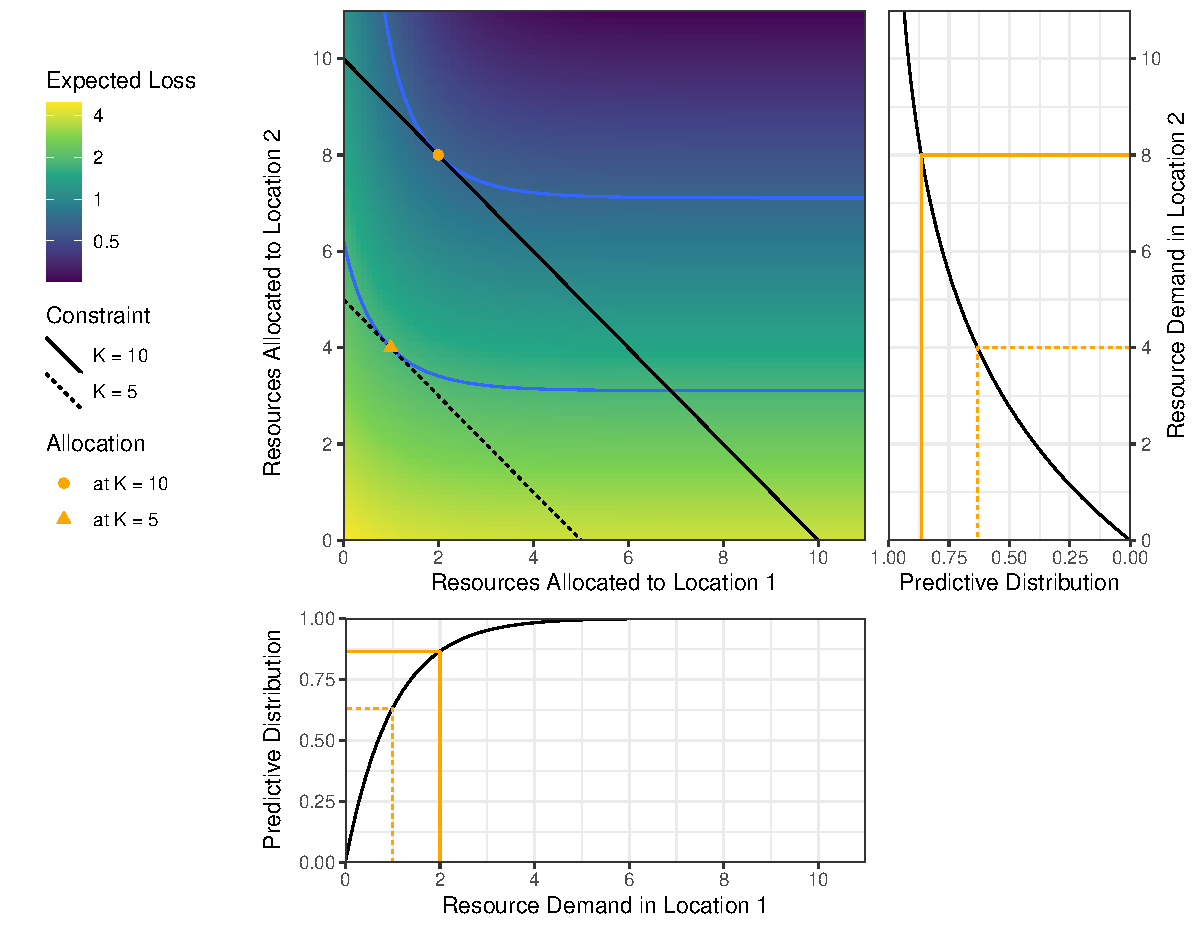
\includegraphics[width=\textwidth]{../figures/exponential_pred_expected_loss.pdf}
    \caption{An illustration of the resource allocation problem in Example 1. There are $N = 2$ locations, with
    predictive distributions $F_1 = \mathrm{Exp}(1)$ and $F_2 = \mathrm{Exp}(1/4)$. The cumulative distribution
    functions of these distributions are illustrated in the panels at bottom and right. In the center panel, the
    background shading corresponds to the expected loss according to these forecasts. Diagonal black lines indicate
    resource constraints at $K=5$ and $K=10$ units; any point along those lines corresponds to an allocation that meets
    the resource constraint. For these forecasts, the optimal allocations are $(1, 4)$ for $K=5$ and $(2, 8)$ for
    $K=10$. These allocations are at the point on the constraint line where the expected loss is smallest, which also
    corresponds to the point where a level set of the expected loss surface (blue curve) is tangent to the constraint.}
    \label{fig:exp_alloc_example}
\end{figure}

Next suppose that we observe resource needs of 1 and 10 in locations 1 and 2, respectively. Based on these observed
needs, we evaluate the allocation suggested by the forecast by calculating the amount of unmet need that resulted from
that allocation over and above what was unavoidable given the resource constraint. With $K = 5$ available resource
units, the allocation based on the forecast exactly meets the observed need in location 1, but it leaves 6 units of need
unmet in location 2. But these 6 units of unmet need are unavoidable under the constraint $K=5$: allocating 0 units of
resources to location 1 and 5 to location 2, for example, still results in a total unmet need of 6 across both
locations. This gives an allocation score of 0 for the forecast when $K = 5$. On the other hand, when $K = 10$, the
forecast's allocation results in $10 - 8 = 2$ units of unmet need in location 2 despite leaving no need unmet in
location 1. In this case, the oracle would be able to prevent all but 1 of the total 11 units of need from going unmet,
for example by allocating 1 unit of resources to location 1 and the remaining 9 units of resources to location 2. So for
$K = 10$, the forecast gets an allocaton score of 1 (= 2 realized $-$ 1 unavoidable) in units of avoidable unmet need.

These scores illustrate a general result: allocation scores for a forecast will tend to be larger when the resource
constraint is close to the observed need, because this is when it matters most which locations are allocated more or
less resources. If the amount of available resources is small relative to the observed need, any allocation of those
limited resources will result in a large amount of unmet need. If the amount of available resources is comparatively
large, it becomes less important which locations receive relatively more or fewer resources because all locations are
likely to
receive enough resources to meet their need. In either of these extremes of resource availability, the avoidable unmet
need that arises from the allocation suggested by a forecast (i.e., the forecast's allocation score) will tend to be
small.

\paragraph{Example 2} \label{examp2} Now consider a different forecast that also has exponential distributions for resource need in
each location, but that has the scale parameters $\sigma_1 = 2$ and $\sigma_2 = 8$, twice as large as the scale
parameters of the forecast in Example 1. Because the optimal allocation is proportional to the scale parameters, this
forecast would lead to the same allocations as the forecast in Example 1, and would therefore be assigned the same
allocation score.

Examination of these results leads to two observations. First, the reason that these forecasts had a positive (i.e.,
non-optimal) allocation score at $K=10$ is that they did not get the relative magnitude of resource need across the two
locations right: the realized need was 10 times as large in location 2 as in location 1, but the forecasts only
indicated that the resource allocation for location 2 should be 4 times the allocation for location 1. At its core, the
allocation score measures whether the forecast accurately captures the relative magnitudes of resource need across
different locations, which is precisely the information that is needed to allocate resources to those locations subject
to a fixed resource constraint.

A second observation is that the forecasts in examples 1 and 2 predicted different mean levels of resource needs, but
had the same allocation score. The allocation score does not directly measure whether the forecasts correctly capture
the absolute magnitude of resource need in each individual location. This stands in contrast to other common scoring
methods that aggregate scores such as log score, CRPS, or WIS for each location, where a poor forecast for one location
is penalized regardless of alignments in other units.

\subsection{A decision theoretic development of the allocation score}
\label{sec:methods.detailed}

We give a high-level review of a general procedure for developing proper scoring rules that are tailored to specific
decision making tasks in section \ref{sec:methods.detailed.decisiontheory}, and then in section
\ref{sec:methods.detailed.specific_allocation} we apply that procedure to develop the allocation score based on the task
of deciding on how to allocate a fixed supply of resources across multiple locations. In
\ref{sec:methods.detailed.integrated_allocation} we consider a small extension where the resource constraint is not
known, or it is desired to consider the value of forecasts across a range of decision making scenarios. This gives rise
to the \emph{integrated allocation score}.

\subsubsection{The decision theoretic setup for forecast evaluation}
\label{sec:methods.detailed.decisiontheory}

Decision theory investigates how decisions are made by formalizing a decision as the process of selecting an
\emph{action} $x$ from a specified set $\mathcal{X}$ of potential actions while taking into consideration the possible
consequences of $x$ under future states of the world. Let $Y$ be a quantifiable aspect of the future which will help to
determine the consequences of $x$. $Y$ is a random variable inasmuch as it is indeterminate when the decision is made.
We refer to a realization $y$ of $Y$ as an \emph{outcome}. A fundamental strategy in decision theory is to assume that
the consequences of an action $x$ under outcome $y$ can be assigned a numeric value, or \emph{loss}, measuring the (lack
of) success of $x$.

Some examples of actions are levels of investment in measures designed to mitigate severe disease outcomes such as
hospital beds, ventilators, medication, or medical staff, with $\mathcal{X}$ being the set of all feasible levels of
investment. An outcome $y$ determining the consequences of such an action might be the number of individuals who
eventually become sick and would benefit from the mitigation measure. In our example, $x$ will succeed to the extent
that it meets the realized need $y$, so that greater unmet need will incur greater loss.

When a forecast $F$ of $Y$ is available, a decision maker might choose that action $x$ which yields the lowest expected
loss according to $F$. The loss of the action $x$ chosen according to $F$ can then, in turn, be interpreted as the value
of $F$ as an input to the decision making process under the realized outcome $y$ of $Y$.

The strategy of minimizing the expected loss according to $F$ might be used if the decision maker trusted that $F$ was
accurate and did not have any additional information that was not captured in $F$. However, here we use it only as a
device for evaluating forecasts by examining the consequences of hypothetical decisions that would be made when using
only $F$ as an input. We return to this point in the discussion.

We arrive at a three-step procedure for developing scoring rules for probabilistic forecasts:
\begin{enumerate}
  \item Specify a \emph{loss function} $s(x, y)$ that measures the loss associated with taking action $x$ when outcome $y$
    eventually occurs.
  \item Given a probabilistic forecast $F$, determine the \emph{Bayes act} $x^F$ that minimizes the expected loss under
    the distribution $F$.
  \item The \emph{scoring rule} for $F$ calculates the score as the loss incurred when the Bayes act was used: 
    $S(F, y) = s(x^F, y)$.
\end{enumerate}
This is a general procedure that may be applied in settings where it is possible to specify a quantitative loss
function. We call a scoring rule obtained from this procedure a \emph{Bayes scoring rule} (noting that to our knowledge, 
this terminology is not standard).  In appendix \ref{sec:a:proper} we review the
result from the scoring rule literature (e.g., \cite{dawid2007geometry,gneiting2007strictly}) that Bayes scoring
rules are proper by construction.

\subsubsection{The allocation score for a fixed resource constraint}
\label{sec:methods.detailed.specific_allocation}

In our setting an action is a vector $x = (x_1, \ldots, x_N)$ specifying the amount of resources allocated to each of
$N$ locations. We require that each $x_i$ is non-negative, and that the total allocation across
all locations equals the amount of available resources, $K$: $\sum_{i=1}^N x_i = K$. The set $\mathcal{X}$ consists of
all possible allocations that satisfy these constraints. The eventually realized resource need in each location is
denoted by $y = (y_1, \ldots, y_N)$; this is a realization (unknown at the
time of decision making) of the random vector $Y = (Y_1, \ldots, Y_N)$. A forecast of the random need $Y$ for each
location is written as $F = (F_1, \ldots, F_N)$. We assume need is non-negative and that the forecasts reflect that, i.e. the
support of each $F_i$ is a subset of $\mathbb{R}^+$. Finally, we assume that each unmet unit of need in any location
incurs a fixed loss of $L>0$, so that if the selected resource level $x_i$ in location $i$ is less than the realized
need $y_i$, a loss of $L \cdot (y_i - x_i)$ results. A variety of extensions to this setup are possible; for example, we
might account for storage costs for resources that go unused, allow for a different loss per unit of unmet need in each
location, or account for resource transportation costs. In this work, we choose to keep the loss function relatively
simple to focus on the core ideas.

It is helpful to clearly distinguish between the time $t_d$ when a decision is made about a public health
resource allocation and the time $t_r$ when resource needs that might be addressed by that allocation occur. Our
setup assumes that $t_d < t_r$ and that the resource in question can only meet the need realized at $t_r$, not prevent
it. That is, we stipulate that the choice of allocation $x$ has no effect on the distribution of the random vector $Y$. In the
context of infectious disease, this means that we do not consider resources, such as vaccines, that are intended to
reduce the number of people who will become sick at some point in the future. Instead, our setup addresses resources
like hospital beds, oxygen supply, or ventilators which are intended to meet the medical needs of patients who are
already sick. Additionally, our setup addresses decision-making that is related to resource needs only at the time
$t_r$; we do not consider sequences of multiple decisions that are made over time or account for the impact of decisions
on resource needs at any time other than $t_r$. We outline some opportunities to extend our work to more complex
decision making settings in the discussion.

With this problem formulation in place, we can develop a proper scoring rule following the procedure in section
\ref{sec:methods.detailed.decisiontheory}.

\paragraph{Step 1: Specify a loss function.} The loss incurred by an allocation $x$ under an outcome $y$ is the sum of
contributions from unmet need in each location:
\begin{equation}
  s_A(x, y) = \sum_{i=1}^N L \cdot \max(0, y_i - x_i). \label{eqn:loss_fn}
\end{equation}
Here, $\max(0, y_i - x_i)$ is the unmet need in location $i$, which is given by $y_i - x_i$ if the realized need $y_i$
in location $i$ is greater than the amount $x_i$ allocated to that location, or $0$ if the amount $x_i$ allocated to
unit $i$ is greater than or equal to the realized need. Also, $L$ is a constant scalar value, the same across all
locations, specifying the ``cost'' of one unit of unmet need.

\paragraph{Step 2: Given a probabilistic forecast $F$, identify the Bayes act.} The Bayes act associated with the
forecast, $x^{F,K}$, is the allocation that minimizes the expected loss, that is, the solution of the \emph{allocation
problem} associated with $K$:
\begin{align}
  \underset{0 \leq x}{\mathrm{minimize}}\,\, \mathbb{E}_{F} [s_A(x, Y)] \text{ subject to }
  \, \sum_{i=1}^N x_i = K, \label{eqn:AP}
\end{align}
where $\mathbb{E}_{F} [s_A(x, Y)] = \sum_{i=1}^{N} L \cdot \mathbb{E}_{F_i}[\max(0, Y_i - x_i)]$ sums the expected loss
due to unmet need across all locations.

In appendix \ref{sec:a:bayes-quantiles} we show that the components of the Bayes act are quantiles 
$x_i^{F,K} = F_i^{-1}(\tau^{F,K})$ at a probability level $\tau^{F,K}$ that depends on the forecast $F$ and the resource
constraint $K$, but is shared across all locations. This probability level is the level at which the resource constraint
is satisfied: $\sum_{i=1}^N F_i^{-1}(\tau^{F,K}) = K$. This tells us that in order to allocate optimally (according to
$F$), we must divide resources among the locations so that there is an equal forecasted probability in every location
that the allocation is sufficient to meet resource need. This solution to the allocation problem is well-known in
inventory management and is often attributed to \cite{hadleywhitin1963}.

\paragraph{Step 3: Define the scoring rule.} We can now use the Bayes act to define a proper scoring rule for the
probabilistic forecast $F$. Consider first the raw score defined as
\begin{align}
  S_A^{\text{raw}}(F, y; K) = s_A(x^{F,K}, y) = \sum_{i=1}^N L \cdot \max(0, y_i - x_i^{F,K}). \label{eqn:AS-raw}
\end{align}
This measures the total unmet need across all locations that results from using the Bayes allocation associated with the
forecast $F$ when the actual level of need in each location is observed to be $y_i$.

To make this a more easily interpreted measure of forecast performance, we will adjust the raw score by subtracting the
minimum loss achievable by an \emph{oracle} allocator which has precise foreknowledge of the outcomes $y_i$. When the
oracle has sufficient resources to meet the total need, i.e., when $\sum_{i=1}^{N}y_i \leq K$, the oracle's loss is zero
and allocation score coincides with the raw score. On the other hand, when the oracle cannot cover all need and incurs a
loss of $L \cdot \left(\sum_{i=1}^{N}y_i - K \right) > 0$, we adjust the raw score by this loss.
The oracle-adjusted score can therefore be written as
\begin{align}
  S_A(F, y; K)  &= S_A^{\text{raw}}(F, y; K) - L \cdot \max\left(0,\sum_{i=1}^{N}y_i - K\right) \\
  &= L\left\{\sum_{i=1}^N \max(0, y_i - x_i^{F,K}) -  \max\left(0,\sum_{i=1}^{N}y_i - K\right)\right\}. \label{eqn:AS-orc}
\end{align}
The oracle adjustment aligns with a common theme in economic decision theory that opportunity loss (often known
as regret or (negative) relative utility) is often a more important quantity than absolute loss (see e.g.,
\cite{DIECIDUE201788}).

\subsubsection{Integrating the allocation score across resource constraint levels}{}
\label{sec:methods.detailed.integrated_allocation}

The allocation score $S_A$ developed in the previous section evaluates the forecast distributions
$F$ based on a single probability level $\tau^{F,K}$. This is appropriate if the resource constraint $K$ is a known
constant. However, if $K$ is not precisely known at the time of decision making or there is interest in measuring the
value of forecasts across a range of decision making scenarios with different resource constraints, we can use an
\emph{integrated allocation score} (IAS) that integrates the allocation score across values of $K$, weighting by a
distribution $p$:
\begin{equation}
S_{IAS}(F, y) = \int S_A(F,y; K) p(K) \, dK \label{eqn:IAS_definition}
\end{equation}
We note that the device of considering a range of hypothetical decision makers or decision making problems with
different problem parameters has been employed in the past \cite[e.g.,][]{murphy1993whatisagoodforecast}.

In practice, it may be challenging to compute the integral in \eqref{eqn:IAS_definition}.
In the applied investigations below we resort to a discretization, evaluating at a grid of values of the resource constraint $K$.
A discrete treatment along these lines will often be natural, in settings where the resource in question is non-divisible (e.g., ventilators, masks).

\subsection{Comparisons with Other Scores}
\label{sec:methods.related}

The weighted interval score (WIS) was proposed in 2020 as a way to score forecasts that were being made in the early
stages of the COVID-19 pandemic \citep{bracher2021evaluating}; equivalent scores had also been used in previous forecast
evaluation efforts \cite[e.g.,][]{hong2016probabilisticEnergyForecasting}. The WIS is a proper scoring rule for
forecasts that use a set of quantiles to represent a probabilistic forecast distribution. Scores are calculated as a weighted sum of
interval scores at different probability levels (e.g., 50\% prediction intervals, 80\% PIs, 95\% PIs, etc...). Larger
interval scores indicate less skillful forecasts. An interval score consists of (a) the width of the interval, with
larger intervals receiving higher scores (higher scores indicate less accuracy), and (b) a penalty if the interval does
not cover the eventual observation, which increases the further away the interval is from the observed value.
Equivalently, the WIS can also be characterized as a weighted sum of quantile scores for each individual predictive
quantile. The quantile score for a particular quantile level assigns an asymmetric penalty to predictions that are too
high or too low, with the relative sizes of the penalties set so that in expectation the score is minimized by the given
quantile of the distribution. The most commonly used version of WIS is one that uses an equal weighting of all quantile
levels, in which case WIS approximates the continuous ranked probability score (CRPS), a commonly used score for
probabilistic forecasts. It is important to note that this weighting was proposed because the resulting score
approximates the CRPS, and not because it aligned with any particular public health decision-making rationale. For more mathematical detail on the WIS, we point readers to \cite{bracher2021evaluating}.

That said, the quantile score and WIS can be derived using the same decision theoretic procedure that we outlined in
section \ref{sec:methods.detailed}. In fields such as meteorology and supply chain management, a great deal of attention
has been given to the problem where a decision must be made about the quantity of a resource to purchase for a single
location in the face of a fixed cost $C$ for each unit of the resource and a loss $L$ that will be incurred for each
unit of unmet need. This leads to the quantile score for the probability level $\tau = 1 - C/L$. From this point, the
WIS or CRPS can be obtained by averaging across a range of decision making settings with different cost and loss
parameters, using a similar motivation that we used to obtain the IAS from the AS in section
\ref{sec:methods.detailed.integrated_allocation} \citep{gneiting2011weightedScoringRules}.

We also note that the AS, just as the (aggregate or mean) quantile score and WIS, depends only on the marginal distributions for each location of a multi-location forecast (see equations \eqref{eqn:AS-raw} and \eqref{eqn:quantiles-sum-to-K} in Section \ref{sec:a:bayes-quantiles} of the appendix). It is however the case that when a forecaster modifies a single marginal forecast (holding those for other locations fixed), the aggregate WIS of their forecast will change only according to the WIS of that marginal forecast, whereas every term in the sum defining the AS (in \eqref{eqn:AS-raw}) will change as the Bayes probability level defined by \eqref{eqn:quantiles-sum-to-K} changes.  In this sense, the AS depends “jointly” on the marginal forecasts while the WIS does not.

\section{Evaluating forecasts of COVID hospitalizations using the allocation score}
\label{sec:application}

We illustrate our new forecast evaluation framework with an application to hospital admissions in the U.S., considering
a hypothetical problem of allocating a limited supply of medical resources to states.

\subsection{Data}
\begin{Schunk}
\begin{Sinput}
> metadata <- tar_meta()
\end{Sinput}
\end{Schunk}

The US COVID-19 Forecast Hub collected short-term forecasts of daily new hospital admissions for individuals with
COVID-19 starting in December 2020 \citep{cramer_united_2022}. The target data for these forecasts were hospital
admissions as reported by the US Department of Health and Human Services through the HealthData.gov website. Forecasts
were probabilistic predictions of the number of new hospital admissions on a particular day in the future, in a specific
jurisdiction of the US (national level, state, or territory). Probability distributions were represented using a set of
23 quantiles for each individual prediction, including a median and the lower and upper limits of 11 central prediction
intervals, from a 99\% to a 10\% prediction interval.

The analysis in this work focuses on forecasts made before and during the first wave of the Omicron SARS-CoV-2 variant
in the US. As such, we analyzed forecasts for the 15 weeks starting with Monday November 22, 2021 through Monday
February 28, 2022.

Submission to the Forecast Hub followed a weekly cycle, and each Monday the Hub collected the most recent forecasts
submitted by all teams that met certain inclusion criteria and created ensemble forecasts using quantile averaging
\citep{ray_comparing_2023}. Our analysis includes these ensembles (\texttt{COVIDhub-ensemble} and
\texttt{COVIDhub-trained\_ensemble}) as well as one other ensemble of hub models created by another team
(\texttt{JHUAPL-SLPHospEns}) and several other individual models. Models were eligible to be included in the analysis if
they were designated as a ``primary'' model from a team. For a model to have a complete, eligible submission in a given
week, it had to have a 14 day-ahead forecast for all 50 states plus Washington DC. Models had to have a complete
forecast for at least 4 of the 15 weeks in the analysis to be eligible for inclusion.

\begin{Schunk}
\begin{Sinput}
> download_date <- format(as.Date(metadata$time[which(metadata$name == "truth_data")]), "%B %d, %Y")
\end{Sinput}
\end{Schunk}

The hospitalization data used for scoring forecasts were downloaded on .

\subsection{Evaluation metrics}

We evaluated forecasts using the allocation score (AS) and the weighted interval score (WIS), computed at a horizon of
14 days. We chose to focus much of our analysis on the AS computed for a resource constraint of $K=15,000$. This level
provides an anchor for interesting comparisons between phases of the Omicron wave by representing a national shortage at
the peak and a national excess before and after the wave (see Figure \ref{fig:metrics-over-time}A), assuming that the
resource need corresponds directly to new hospital admissions. We additionally computed the mean WIS (MWIS) across all
of the forecasted state-level locations. 

For both scores, we also computed standardized ranks among all models that submitted forecasts each week. The
standardized rank lies in the interval $[0, 1]$, where 0 corresponds to the worst rank and 1 to the best. In the case of
a tie between one or more models, all models received the better rank.

As described above, predictions were submitted to the Forecast Hub in the form of a set of 23 quantiles of the
predictive distribution. The WIS can be directly calculated from these quantiles. However, our numerical method for calculating 
the AS (outlined in appendix \ref{sec:a:numeric})
requires a full cumulative distribution function (CDF) for the forecast in each location.
For the purpose of this analysis, we imputed CDFs based on the provided quantiles following a procedure detailed in 
appendix \ref{sec:a:distfromq}. Briefly, this involves interpolating the provided quantiles between the lowest (.01) and highest 
(.99) probability levels using monotonic cubic splines, and then extending outside these levels with normal distribution tails
parametrized to match the two lowest and two highest quantiles. We show in appendix \ref{sec:a:propriety_of_parametric_approximation}
that if this evaluation procedure
had been specified prospectively, the resulting score would be proper, but that a post hoc application of this
procedure is improper. We use the procedure here to illustrate the properties of the AS, and note that a collaborative
forecasting hub interested in using the AS for evaluation could circumvent propriety issues by communicating the
definition of the AS to forecasters and then collecting allocations at specified resource levels as part of forecast
submissions.

\subsection{Allocation benchmarks}

In order to explore how model-derived allocations might be compare to ``standard operating procedures'' for allocation
used by public health officials, we scored two simple benchmark methods. First, we evaluated forecasts from the
\texttt{COVIDhub-baseline} model, which predicts a flat line from the most recent observation with uncertainty bounds
based on a random walk \citep{cramer_evaluation_2022}. Second, we generated a proposed set of allocations where the
quantity allocated to each state was proportional to that state's population (using US Census data of vintage 2022
\citep{us_census_nst_est2022}), referred to below as \texttt{per-capita}. These two approaches generally reflect common
choices for ``best practices'' of allocation: either allocating resources based on the most recent observed data, or in
proportion to the population of each location. 

\subsection{Data and code availability}

All forecast data used in this evaluation are available through the COVID-19 Forecast Hub \citep{cramer_united_2022}. An
R package implementing the allocation score is available at \url{https://github.com/aaronger/alloscore}. All code and
data for the analyses presented in this manuscript are available at
\url{https://github.com/aaronger/utility-eval-papers}. The analyses were generated using a reproducible workflow using
R version 4.5.1 (2025-06-13) and the {\tt targets} package \citep{Rcore-2023, landau_2021_targets}.

\subsection{Application results}

\begin{Schunk}
\begin{Sinput}
> tar_load("Kat15k_alloscores")